\documentclass[12pt]{article}

\usepackage{adjustbox}
\usepackage{amssymb}
\usepackage{amsmath}
\usepackage{amsfonts} 
\usepackage{array}
\usepackage{colortbl}
\usepackage{fancyhdr}
\usepackage[colorlinks=true, urlcolor=blue, linkcolor=black]{hyperref}
\usepackage{lastpage}
\usepackage[margin=1in, bottom=1.07in]{geometry} 
\usepackage{mathtools}
\usepackage{pgf}
\usepackage{pgfplots}
\usepackage{pgf-pie}
%\usepackage{pgfplotstable}  
\usepackage{tikz}
\usepackage{xcolor}
\usepackage{graphicx}
\usepackage{multirow}
\usepackage{pbox}
\usepackage{xltabular}

\graphicspath{{C:/Users/neil.rogers/OneDrive - afacademy.af.edu/figures}}

\newcommand\thesemester{Spring 2025}
\newcommand\theclass{ECE 343}
\newcommand{\rot}[1]{\multicolumn{1}{c}{\adjustbox{angle=60,lap=\width-1em}{#1}}} % rotated column headers
\def\yes{$\color{green!50!black} \checkmark$} % green checkmarks

% set headers and footers
\pagestyle{fancy}
\fancyhead[R]{\includegraphics[scale=0.2]{USAFA-logo}}
\fancyhead[L]{\rule[-2ex]{0pt}{2ex}\includegraphics[scale=0.03]{DFEC-logo}}
%\fancyfoot[C]{\theclass \hspace{1pt} -- \thesemester}
\fancyfoot[L]{{\theclass} - {\thesemester}}
\fancyfoot[C]{}%\thesemester}
\fancyfoot[R]{\thepage\hspace{1pt} of\hspace{1pt} \pageref{LastPage}}
\setlength{\headsep}{54pt}
\setlength{\parskip}{10pt}
\setlength{\itemsep}{4pt}
\setlength{\topsep}{4pt}
\setlength{\parindent}{0pt}
\setlength{\footskip}{12pt}
\renewcommand{\footrulewidth}{0.5pt}
\renewcommand{\headrulewidth}{0.5pt}
\def\hdrpad{12pt}

% for the plain first page
\fancypagestyle{plain}{
\fancyhf{}
\setlength{\headsep}{0pt}
\renewcommand{\headrulewidth}{0pt}
\renewcommand{\footrulewidth}{0pt}
}

\begin{document}

\thispagestyle{plain}
\begin{minipage}[c]{0.15\textwidth}
\begin{center}
%\includegraphics[scale=0.3]{USAFA-logo} \hspace{12pt}%
\includegraphics[scale=0.05]{DFEC-logo}\\[6pt]
\end{center}
\end{minipage}%
\begin{minipage}[t]{0.85\textwidth}
%\begin{center}
%DEPARTMENT OF ELECTRICAL AND COMPUTER ENGINEERING \\
\begin{flushright}\begin{Large}\textbf{ECE 343: Intro to Electromagnetics}\end{Large} \\[6pt]
\begin{large} {\color{blue}{\textbf{\thesemester}}} \end{large} \\[6pt]
\end{flushright} 
\end{minipage}

\setlength{\unitlength}{1in}

\begin{picture}(6,.1) 
\put(0,0) {\line(1,0){6.5}}         
\end{picture}

 
\vspace{12pt}
\textbf{Course description}  
	
At its core, electromagnetics is the study of wave propagation. How do electromagnetic waves differ from the classical understanding of circuits? If they are indeed different, how do we deal with that and use it to our advantage? How does this fundamental understanding of electromagnetics enable key aspects of modern life?  An understanding of electromagnetics is a crucial part of any Electrical Engineer's toolset; in this course, we will explore wave propagation to answer some of these questions \&  more. 

\textbf{Instructor} 

\vspace{-12pt}

	\begin{minipage}[t]{0.85\textwidth}
		\begin{flushleft}
		\begin{tabular}{l l l}
		Dr. Neil Rogers (Course Director) & 2E38 &\href{mailto:neil.rogers.1@afacademy.af.edu}{neil.rogers.@afacademy.edu} \\
		\end{tabular}
		\end{flushleft}
	\end{minipage}%
	\begin{minipage}[c]{0.15\textwidth}
		\href{https://bit.ly/3BFvEPa}{\includegraphics[scale=0.08]{EIQR}}
	\end{minipage}
	
\textbf{Course Goals}

	Cadets enrolled in the course shall develop the ability to analyze and understand electrostatics, magnetostatics, and electromagnetic-wave propagation and their roles in modern electronic systems.

\textbf{Course Objectives}
	\vspace{-12pt}
	\begin{enumerate}
		\item Solve transmission-line problems using their knowledge of electromagnetics to include impedance matching techniques, circuit parameters and the Smith chart.
		\item Explain the meaning of Maxwell’s equations, in both static and dynamic situations and apply them to the study of electromagnetics
		\item Set-up and solve electromagnetic propagation problems.
	\end{enumerate}
	\vspace{-12pt}

\textbf{Course Prerequistes} 
\vspace{-12pt}
\begin{itemize}
	\item \textbf{Physics 215:} Coulomb, Faraday, Ampere,  Gauss’ laws.
	\item \textbf{ECE 346:} Divergence, gradient, curl, including divergence theorem and Stoke’s theorem, partial differential equations (specifically separation of variables).
\end{itemize}
	
\textbf{Course Text} 

Ellingson, Steven W. (2018) Electromagnetics, Vol. 1. Blacksburg, VA: VT Publishing. \href{https://doi.org/10.21061/electromagnetics-vol-1}{https://doi.org/10.21061/electromagnetics-vol-1} CC BY-SA 4.0

%%%%%%%%%%%%%%%%%%%%%%%%%%%%%%%%%%%%%%%%%%%%%%%%%%%%%%%%%%%%%%%%%
%%%%%%%%%%%%%%%%%%%%%%%%%%%%%%%%%%%%%%%%%%%%%%%%%%%%%%%%%%%%%%%%
\newpage
\fancyhead[C]{\Large\textbf{Grading}}

\begin{small} 
Grades in this course will be assigned based on your \textbf{mastery} of learning objectives, \textbf{engagement} in course material, and traditional \textbf{exams}. 
\end{small}

\vspace{-0.1in}

\begin{minipage}[c]{0.55\textwidth}

%\vspace{-1in}

	\center\textbf{\hspace{0.15in}Prog Grade Weighting}
	
	\vspace{12pt}
	
	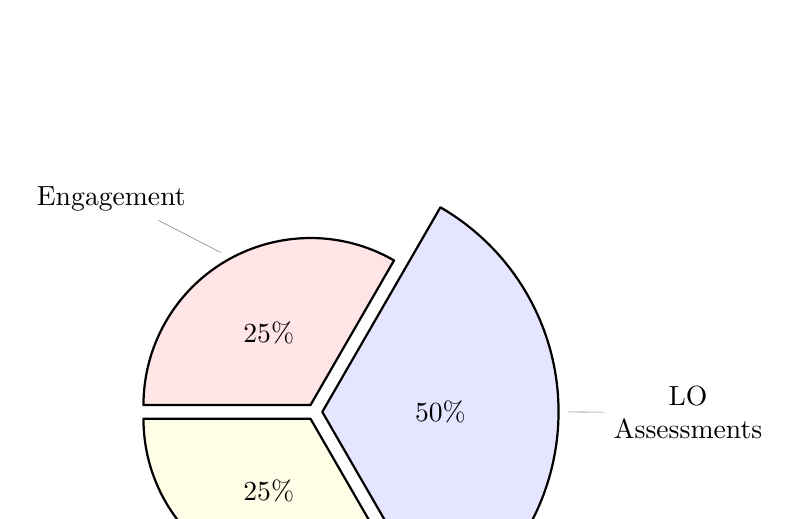
\begin{tikzpicture}[scale=1]
		\pie[/tikz/every pin/.style={align=center}, 
				text=pin,
				rotate=180, 
				polar,
				explode=0.1,
				color={yellow!10!white, blue!10!white, red!10!white}
				]
				 {25/GR, %
				   50/{LO \\ Assessments}, %
				   25/Engagement
							      }
	\end{tikzpicture}

	\vspace{0.25in}
	
	\center\textbf{\hspace{0.15in}Final Grade Weighting}

	\vspace{12pt}

	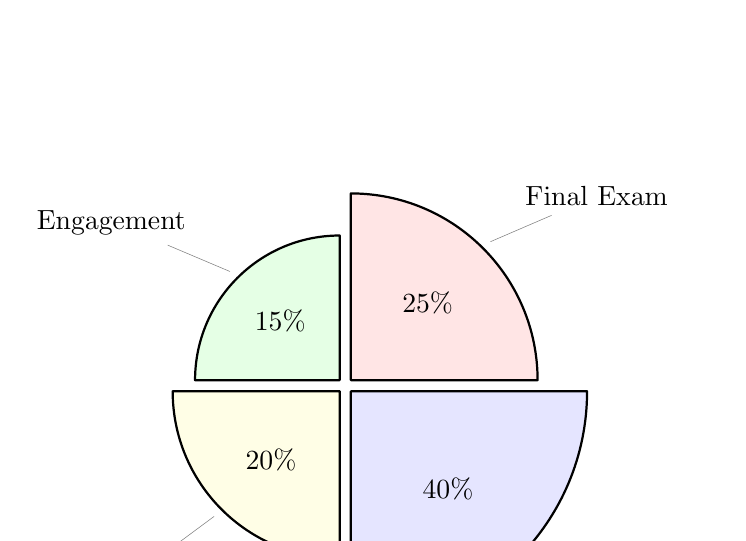
\begin{tikzpicture}[scale=1]
			\pie[/tikz/every pin/.style={align=center}, 
				text=pin,
				rotate=180, 
				polar,
				explode=0.1,
				color={yellow!10!white, blue!10!white, red!10!white, green!10!white}
				] 
				 {20/GR , %
		                40/{LO \\ Assessments}, %
		                25/Final Exam, %
		                15/Engagement
							      }
	\end{tikzpicture}%
\end{minipage}%
\hspace{\fill}%
\begin{minipage}[c]{0.35\textwidth}
\begin{footnotesize}
\begin{tabular}{|p{\textwidth}}
	

	 \textbf{Assessments} will be given for each learning objective. Assessments are graded on a binary scale, based on demonstrated mastery. Earning a 1 on an assessment indicates mastery of the associated learning objective. Earning a  indicates you have not yet mastered the learning objective. You may revise your work, based on the detailed feedback, unless no effort is evident (the assessment is blank, incomplete, or significantly late); then you will not be allowed a retake. A retake may be earned by giving a 5 minute technical presentation during class on a relevant topic.\\
	
	\\
	
	 \textbf{GRs and the Final Exam} are individual efforts. The GR will be taken out of class and will be graded on a specification scale of: 0, 0.5, and 1 for each problem. The final exam will be taken during the assigned period during finals week and will be graded similarly.  \\
	
	\\
	
	\textbf{Engagement Credits (EC)} You may earn engagement points by engaging with the course content in the following ways:
	\begin{itemize}
		\item Completing \textbf{Practice problems}
		\item Attending \textbf{EI}
		\item Up to 5 engagement points may be earned for completing a \textbf{research paper} on a relevant, pre-approved topic. The paper must be in IEEE format, contain at least 3 scholarly references, and adhere to submission standards contained in this syllabus.
	\end{itemize}
	
\end{tabular}	
\vspace{-0.1in}
\end{footnotesize}
\end{minipage}

\vspace{-0.12in}

\begin{center}
%\textbf{\Large Grade Scale}

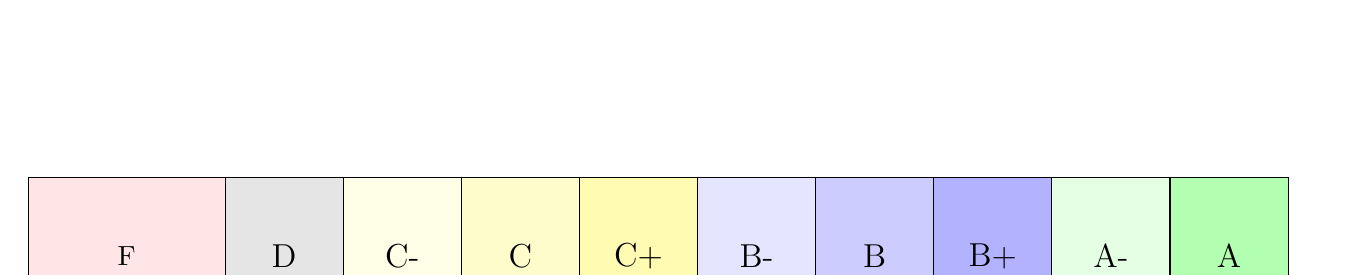
\begin{tikzpicture}[scale=1]
	\draw (-2.5cm,0) rectangle ++(13.5cm,2cm);
	\draw[fill=red!10!white] (-2.5cm, 0) rectangle ++ (2.5cm,2cm); % F
	\draw[fill=black!10!white] (0,0) rectangle ++(1.5cm,2cm); % D
	\draw[fill=yellow!10!white] (1.5cm,0cm) rectangle ++(1.5cm,2cm); % C-
	\draw[fill=yellow!20!white] (3cm,0cm) rectangle ++(1.5cm,2cm); % C
	\draw[fill=yellow!30!white] (4.5cm,0cm) rectangle ++(1.5cm,2cm); % C+
	\draw[fill=blue!10!white] (6cm,0cm) rectangle ++(1.5cm,2cm); %B-
	\draw[fill=blue!20!white] (7.5cm,0cm) rectangle ++(1.5cm,2cm); % B
	\draw[fill=blue!30!white] (9cm,0cm) rectangle ++(1.5cm,2cm); % B+
	\draw[fill=green!10!white] (10.5cm,0cm) rectangle ++(1.5cm,2cm); %A-
	 \draw[fill=green!30!white] (12cm,0cm) rectangle ++(1.5cm,2cm); % A
	\node at (-1.25cm, 1cm) {F};
	\node at (0cm,-0.5cm) {{$\leq$} 60\%};
	\node at (0.75cm, 1cm) {\large D};
	\node at (1.5cm,-0.5cm) {70\%};
	\node at (2.25cm, 1cm) {\large C-};
	\node at (3cm,-0.5cm) {73\%};
	\node at (3.75cm, 1cm) {\large C};
	\node at (4.5cm,-0.5cm) {77\%};
	\node at (5.25cm, 1cm) {\large C+};
	\node at (6cm,-0.5cm) {70\%};
	\node at (6.75cm, 1cm) {\large B-};
	\node at (7.5cm,-0.5cm) {83\%};
	\node at (8.25cm, 1cm) {\large B};
	\node at (9cm,-0.5cm) {87\%};
	\node at (9.75cm, 1cm) {\large B+};
	\node at (10.5cm,-0.5cm) {90\%};
	\node at (11.25cm, 1cm) {\large A-};
	\node at (12cm,-0.5cm) {93\%};
	\node at (12.75cm, 1cm) {\large A};
	\node at (13.5cm,-0.5cm) {100\%};
	
\end{tikzpicture}
\end{center}




%%%%%%%%%%%%%%%%%%%%%%%%%%%%%%%%%%%%%%%%%%%%%%%%%%%%%%%%%%%%%%
% Learning Objectives
%%%%%%%%%%%%%%%%%%%%%%%%%%%%%%%%%%%%%%%%%%%%%%%%%%%%%%%%%%%%%%

\newpage
\fancyhead[C]{\Large\textbf{Learning Objectives}}
\def\myfontsize{normalsize}
\renewcommand{\arraystretch}{1.25}
% !TEX root =./Admin/ECE346_Syllabus_Fall 2024.tex

\begin{\myfontsize}

%\renewcommand{\arraystretch}{1.25}
\newcolumntype{b}{X} % big column
%\newcolumntype{m}{>{\hsize=.2\hsize}X} % medium column, .2 width of big
%\newcolumntype{s}{>{\hsize=.1\hsize}X} % small column, .1 width of big
\newcounter{objnum}
\setcounter{objnum}{1}
\newcounter{chapnum}
\setcounter{chapnum}{1}

%-----------------------------------------------------------
\def\chrowcolor{green!10!white}

\begin{center}
\begin{xltabular}{0.9\textwidth}{|c|X |} %columns are sb
\hline
\textbf{Obj}   & \textbf{Description} \\ \hline\hline\endhead % & \textbf{Format}\\ \hline\hline\endhead

\rowcolor{\chrowcolor}\multicolumn{2}{|c|}{Chapter {\thechapnum} - Introduction}
\\ \hline

\thechapnum.\theobjnum
& I can articulate what I will learn and how I will be assessed in this course.
\stepcounter{objnum}
\\\hline

\thechapnum.\theobjnum
& I can articulate practical applications of electromagnetics.
\setcounter{objnum}{1}
\stepcounter{chapnum}
\\\hline

%%%%%%%%%%%%%%%%%%%%%%%%%%%%%%%%%%%%%%%%%%%%%%%%%%%%%%%%%%%%%%%

\rowcolor{\chrowcolor}\multicolumn{2}{|c|}{Chapter {\thechapnum} - Fields}
\\\hline

\thechapnum.\theobjnum
& I can recall the definition of scalar fields, vector fields, phasors, and Euler's identity.
\stepcounter{objnum}
\\\hline 

\thechapnum.\theobjnum
& I can explain the basic terms and quantities used to describe electromagnetic fields. 
\setcounter{objnum}{1}
\stepcounter{chapnum}
\\\hline 

%%%%%%%%%%%%%%%%%%%%%%%%%%%%%%%%%%%%%%%%%%%%%%%%%%%%%%%%%%%%%%%

\rowcolor{\chrowcolor}\multicolumn{2}{|c|}{Chapter {\thechapnum} - Transmission Lines}
\\\hline

\thechapnum.\theobjnum
& I can describe the origin of the transmission line equation, understand the method of developing a solution, and interpret the solution.
\stepcounter{objnum}
\\\hline 

\thechapnum.\theobjnum
& I can explain the physical meaning of and calculate the following quantities: propagation constant, phase constant, attenuation constant, characteristic impedance, VSWR, reflection coefficient, and transmission coefficient.
\stepcounter{objnum}
\\\hline 

\thechapnum.\theobjnum
& I can use the transmission line equation to calculate the voltage/current at an arbitrary point on a specified transmission line.
\stepcounter{objnum}
\\\hline 

\thechapnum.\theobjnum
& I can use the transmission line equation to match a load to a source using a length of transmission line.
\stepcounter{objnum}
\\\hline 

\thechapnum.\theobjnum
& I can identify the various quantities represented on the Smith Chart.
\stepcounter{objnum}
\\\hline 

\thechapnum.\theobjnum
& I can use a Smith Chart to design a matching network for a given source and load, using series components, parallel components, shorted stubs, and open stubs.
\stepcounter{objnum}
\\\hline 

\thechapnum.\theobjnum
&  I can plot the transient response of a load connected to a source through a transmission line.
\stepcounter{objnum}
\\\hline 

\thechapnum.\theobjnum
& I can measure the reflection coefficient across a range of frequencies and interpret the measurement using a network analyzer.
\setcounter{objnum}{1}
\stepcounter{chapnum}
\\\hline 

%%%%%%%%%%%%%%%%%%%%%%%%%%%%%%%%%%%%%%%%%%%%%%%%%%%%%%%%%%%%%%%

\rowcolor{\chrowcolor}\multicolumn{2}{|c|}{Chapter {\thechapnum} - Vector Analysis}
\\\hline

\thechapnum.\theobjnum
& I can recognize and apply common vector calculus operations, such as: gradient, divergence, curl, and Laplacian in the three major coordinate systems.
\stepcounter{objnum}
\\\hline 

\thechapnum.\theobjnum
& I can calculate surface and volume integrals in rectangular, cylindrical, and spherical coordinate systems. 
\stepcounter{objnum}
\\\hline 

\thechapnum.\theobjnum
& I can differentiate between Stoke's Theorem and the Divergence Theorem and apply them to various problems to simplify integrals. \vspace{48pt}
\setcounter{objnum}{1}
\stepcounter{chapnum}
\\ \hline 

%%%%%%%%%%%%%%%%%%%%%%%%%%%%%%%%%%%%%%%%%%%%%%%%%%%%%%%%%%%%%%%

\rowcolor{\chrowcolor}\multicolumn{2}{|c|}{Chapter {\thechapnum} - Electrostatics}
\\\hline

\thechapnum.\theobjnum
&  I can apply Coloumb's Law to use direct integration to calculate the electric field due to charge density in varoius geometries, including rectangular, cylindrical, and spherical coordinate systems. 
\stepcounter{objnum}
\\\hline 

\thechapnum.\theobjnum
&  I can apply the integral and differential forms of Gauss' Law to calculate the electric field due to charge density in various geometries, including rectangular, cylindrical, and spherical coordinate systems. 
\stepcounter{objnum}
\\\hline 

\thechapnum.\theobjnum
&  I can  calculate the electric field from the scalar electric potential in a variety of geometries.
\stepcounter{objnum}
\\\hline 

\thechapnum.\theobjnum
&  I can apply the electric field boundary conditions to calculate electric fields on both sides of a material boundary. 
\setcounter{objnum}{1}
\stepcounter{chapnum}
\\ \hline 

%%%%%%%%%%%%%%%%%%%%%%%%%%%%%%%%%%%%%%%%%%%%%%%%%%%%%%%%%%%%%%%

\rowcolor{\chrowcolor}\multicolumn{2}{|c|}{Chapter {\thechapnum} - Steady Current and Conductivity}
\\\hline

\thechapnum.\theobjnum
&  I can calculate the total current through a surface area given a current distribution. 
\stepcounter{objnum}
\\ \hline 

\thechapnum.\theobjnum
&  I can use Ohm's Law for electromagnetics to calculate the relationship between a current distribution and an electric field. 
\stepcounter{objnum}
\\ \hline 

\thechapnum.\theobjnum
&  I can articulate and identify what makes a material a good conductor and how conductivity relates to resistance. 
\setcounter{objnum}{1}
\stepcounter{chapnum}
\\ \hline 

%%%%%%%%%%%%%%%%%%%%%%%%%%%%%%%%%%%%%%%%%%%%%%%%%%%%%%%%%%%%%%%

\rowcolor{\chrowcolor}\multicolumn{2}{|c|}{Chapter {\thechapnum} - Magnetostatics}
\\\hline

\thechapnum.\theobjnum
&  I can use the Biot-Savart law to simple magnetostatic systems to find the magnetic field at an observation point. 
\stepcounter{objnum}
\\ \hline 

\thechapnum.\theobjnum
&  I can articulate the meaning of both the integral form and point form of Gauss' Law for magnetism.
\stepcounter{objnum}
\\ \hline 

\thechapnum.\theobjnum
& I can use Ampere's Law to calculate the magnetic field at an observation point for simple magnetostatic systems.
\stepcounter{objnum}
\\ \hline 

\thechapnum.\theobjnum
&  I can apply the magnetic field boundary conditions to calculate magnetic fields on both sides of a material boundary.  
\setcounter{objnum}{1}
\stepcounter{chapnum}
\\ \hline 

%%%%%%%%%%%%%%%%%%%%%%%%%%%%%%%%%%%%%%%%%%%%%%%%%%%%%%%%%%%%%%%

\rowcolor{\chrowcolor}\multicolumn{2}{|c|}{Chapter {\thechapnum} - Dynamic Fields}
\\\hline

\thechapnum.\theobjnum
&  I can articulate the significance of the displacement current and calculate it, given a time-varying electric field.
\stepcounter{objnum}
\\ \hline 

\thechapnum.\theobjnum
& I can articulate the meaning of and calculate the relaxation time for a variety of materials. 
\stepcounter{objnum}
\\ \hline 

\thechapnum.\theobjnum
&  I know the forms of Maxwell's equations for time-varying fields and use them to calculate electric and magnetic fields for a variety of physical systems.  \vspace{48pt}
\setcounter{objnum}{1}
\stepcounter{chapnum}
\\ \hline 



%%%%%%%%%%%%%%%%%%%%%%%%%%%%%%%%%%%%%%%%%%%%%%%%%%%%%%%%%%%%%%%

\rowcolor{\chrowcolor}\multicolumn{2}{|c|}{Chapter {\thechapnum} - Plane Waves}
\\\hline

\thechapnum.\theobjnum
&  I understand the process of decoupling and finding solutions for Maxwell's equations for dynamic fields. 
\stepcounter{objnum}
\\ \hline 

\thechapnum.\theobjnum
& I can articulate what a Uniform Plane Wave (UPW) is and describe key properties that relate the electric and magnetic field. 
\stepcounter{objnum}
\\ \hline 

\thechapnum.\theobjnum
&  I can calculate the electric and magnetic fields for a UPW.
\stepcounter{objnum}
\\ \hline 

\thechapnum.\theobjnum
& I can articulate the concept of polarization and determine the polarization for various UPWs.
\stepcounter{objnum}
\\ \hline 

\thechapnum.\theobjnum
& I can determine the reflection and transmission of UPW at a boundary for Transverse Electric (TE) and Transverse Magnetic (TM) waves, using boundary conditions.
\setcounter{objnum}{1}
\stepcounter{chapnum}
\\ \hline 
\end{xltabular}			
\end{center}
\end{\myfontsize}
%-----------------------------------------------------------


%%%%%%%%%%%%%%%%%%%%%%%%%%%%%%%%%%%%%%%%%%%%%%%%%%%%%%%%%%%%%%
% Notional Schedule
%%%%%%%%%%%%%%%%%%%%%%%%%%%%%%%%%%%%%%%%%%%%%%%%%%%%%%%%%%%%%%

\newpage
\fancyhead[C]{\Large\textbf{Course Outline - Prog (Nominal) }}

% Prog
\def\lessonNum{0}
\newcounter{mylnum}
\vspace{12pt}
\renewcommand{\arraystretch}{1.5}
\def\myfontsize{normalsize}

\setcounter{mylnum}{1}
\begin{center}
\begin{\myfontsize}
\begin{tabular}{| c | l | c | l |}
\hline
\textbf{Lesson} 		  	& \textbf{Topics}             & \pbox{5cm}{\textbf{Reading}}	& \textbf{Notes}		\\ \hline\hline
\ifnum\lessonNum=\value{mylnum} \rowcolor{green!20!white}\fi
	\themylnum  
	& Course Overview  \& Introduction		
	& Ch.1 
	&  LO 1.1-1.2 
	\stepcounter{mylnum}\\ \hline \hline
\rowcolor{gray!20!white}\multicolumn{4}{| c |}{\textbf{Chapter 2: Electric and Magnetic Fields}}	\\ \hline\hline
\ifnum\lessonNum=\value{mylnum} \rowcolor{green!20!white}\fi
	\themylnum 	
	& Fields, Parameters, Field Quantities	
	& Ch. 2	
	& LO 2.1-2.2			
\stepcounter{mylnum}\\ \hline\hline
\rowcolor{gray!20!white}\multicolumn{4}{| c |}{\textbf{Chapter 3: Transmission Lines}}	 \\ \hline\hline	
\ifnum\lessonNum=\value{mylnum} \rowcolor{green!20!white}\fi
	\themylnum 	
	& Lumped Element Model				
	& 3.1-3.4 
	& LO 3.1		
\stepcounter{mylnum}\\ \hline
\ifnum\lessonNum=\value{mylnum} \rowcolor{green!20!white}\fi
	\themylnum 	
	& Telegrapher's Equations
	& 3.5-3.6
	&  LO 3.1	
\stepcounter{mylnum}\\ \hline
\ifnum\lessonNum=\value{mylnum} \rowcolor{green!20!white}\fi
	\themylnum 	
	&  Characteristic Impedance \& Wave Propagation	
	& 3.7-3.9		
	& LO 3.2						
\stepcounter{mylnum}\\ \hline
\ifnum\lessonNum=\value{mylnum} \rowcolor{green!20!white}\fi
	\themylnum 	
	& Coaxial,  Reflection Coefficient, VSWR	
	& 3.10,3.12-3.14	
	& LO 3.2-3.3		
\stepcounter{mylnum}\\ \hline 
\ifnum\lessonNum=\value{mylnum} \rowcolor{green!20!white}\fi
	\themylnum 	
	&  Terminated Transmission Lines	
	&  3.15,3.17-3.19
	& LO 3.4		
\stepcounter{mylnum}\\ \hline 
\ifnum\lessonNum=\value{mylnum} \rowcolor{green!20!white}\fi
	\themylnum	
	& Impedance Matching	
	& 3.21-3.23
	& LO 3.4 			
\stepcounter{mylnum}\\ \hline 
\ifnum\lessonNum=\value{mylnum} \rowcolor{green!20!white}\fi
	\themylnum  
	& Impedance Matching	
	& 3.21-3.23
	& LO 3.4		
\stepcounter{mylnum}\\ \hline 
\ifnum\lessonNum=\value{mylnum} \rowcolor{green!20!white}\fi
	\themylnum	
	& Smith Charts
	& Supplemental
	& LO 3.5
\stepcounter{mylnum}\\ \hline 
\ifnum\lessonNum=\value{mylnum} \rowcolor{green!20!white}\fi
	\themylnum	
	& Smith Charts
	& Supplemental 
	& LO 3.5					
\stepcounter{mylnum}\\ \hline 
\ifnum\lessonNum=\value{mylnum} \rowcolor{green!20!white}\fi
	\themylnum	
	& Smith Charts
	& Supplemental 
	& LO 3.5	
\stepcounter{mylnum}\\ \hline 
\ifnum\lessonNum=\value{mylnum} \rowcolor{green!20!white}\fi
	\themylnum	
	& Smith Charts
	& Supplemental 
	& LO 3.5	
\stepcounter{mylnum}\\ \hline 

\ifnum\lessonNum=\value{mylnum} \rowcolor{green!20!white}\fi
	\themylnum	
	& Transients		
	& Supplemental 
	& LO 3.6	 
\stepcounter{mylnum}\\ \hline \hline
\ifnum\lessonNum=\value{mylnum} \rowcolor{green!20!white}\fi
	\themylnum 	
	& Flex Day
	& 
	& 	
\stepcounter{mylnum}\\ \hline 
\ifnum\lessonNum=\value{mylnum} \rowcolor{green!20!white}\fi
	\themylnum 	
	& Reflection/Transmission Coefficient Lab
	& Lab Packet
	& LO 3.7		
\stepcounter{mylnum}\\ \hline 
\ifnum\lessonNum=\value{mylnum} \rowcolor{green!20!white}\fi
	\themylnum 	
	& Reflection/Transmission Coefficient Lab
	& Lab Packet
	& LO 3.7		
\stepcounter{mylnum}\\ \hline 
\rowcolor{gray!20!white}\multicolumn{4}{| c |}{\textbf{Chapter 4: Vector Analysis}} \\ \hline\hline
\ifnum\lessonNum=\value{mylnum} \rowcolor{green!20!white}\fi
	\themylnum	
	& Vector \& Coordinate System Review
	& Ch. 4
	&LO 4.1-4.4 \textbf{GR 1 due}	
\stepcounter{mylnum}\\ \hline 
\rowcolor{gray!20!white}\multicolumn{4}{| c |}{\textbf{Chapter 5: Electrostatics}}\\ \hline\hline
\ifnum\lessonNum=\value{mylnum} \rowcolor{green!20!white}\fi
	\themylnum	
	& Coulomb's Law
	& 5.1-5.3
	& LO 5.1
\stepcounter{mylnum}\\ \hline 
\ifnum\lessonNum=\value{mylnum} \rowcolor{green!20!white}\fi
	\themylnum	
	& Surface and Volume Charge			
	& 5.4
	& LO 5.1
\stepcounter{mylnum}\\ \hline 
\ifnum\lessonNum=\value{mylnum} \rowcolor{green!20!white}\fi
	\themylnum	
	& Gauss' Law (Integral Form)
	& 5.5-5.6
	& LO 5.2		 					
\stepcounter{mylnum}\\ \hline 
\ifnum\lessonNum=\value{mylnum} \rowcolor{green!20!white}\fi
	\themylnum	
	& Gauss' Law (Differential Form)		
	& 5.7-5.8
	& LO 5.2	 	
\stepcounter{mylnum}\\ \hline 
\ifnum\lessonNum=\value{mylnum} \rowcolor{green!20!white}\fi
	\themylnum	
	& Electric Potential	
	& 5.9-5.10, 5.15
	&  LO 5.3	
\stepcounter{mylnum}\\ \hline 
% <---- line 129 should be 20 lessons, based on 6 lines per lesson, starting at line 9 
\end{tabular}			
\end{\myfontsize}
\end{center}


% Final
\newpage
\fancyhead[C]{\Large\textbf{Course Outline - Final (Nominal)}}
\def\lessonNum{0}
\vspace{24pt}
\renewcommand{\arraystretch}{1.5}
\setcounter{mylnum}{24}
%\def\myfontsize{normalsize}
\begin{center}
\begin{\myfontsize}
\begin{tabular}{| c | l | c | l |}
\hline
\textbf{Lesson} 		  	& \textbf{Topics}             & \pbox{5cm}{\textbf{Reading}}	& \textbf{Notes}		\\ \hline\hline
\ifnum\lessonNum=\value{mylnum} \rowcolor{green!20!white}\fi
	\themylnum  
	& BVP (Capacitor, Coax), Electric Potential	
	& 5.16
	&  LO 5.3  
\stepcounter{mylnum}\\ \hline \hline
\ifnum\lessonNum=\value{mylnum} \rowcolor{green!20!white}\fi
	\themylnum 	
	& Electric Boundary Conditions
	& 5.18-5.22	
	& LO 5.4			
\stepcounter{mylnum}\\ \hline
\ifnum\lessonNum=\value{mylnum} \rowcolor{green!20!white}\fi
	\themylnum 	
	& BC's/Capacitance			
	& 5.23-5.24
	& 	
\stepcounter{mylnum}\\ \hline
\ifnum\lessonNum=\value{mylnum} \rowcolor{green!20!white}\fi
	\themylnum 	
	& Electrostatic Lab			
	& Lab packet
	& 	
\stepcounter{mylnum}\\ \hline
\rowcolor{gray!20!white}\multicolumn{4}{| c |}{\textbf{Chapter 6: Steady Current \& Conductivity}}	\\ \hline\hline
\ifnum\lessonNum=\value{mylnum} \rowcolor{green!20!white}\fi
	\themylnum 	
	& Current density, Conductivity, Resistance
	& Ch. 6
	&   					
\stepcounter{mylnum}\\ \hline\hline
\rowcolor{gray!20!white}\multicolumn{4}{| c |}{\textbf{Chapter 7: Magnetostatics}}						\\ \hline\hline
\ifnum\lessonNum=\value{mylnum} \rowcolor{green!20!white}\fi
	\themylnum 	
	&  Magnetic Fields, Gauss' Law for Magnetism	
	& 7.1-7.3		
	&LO 7.1-7.2 \textbf{GR 2} 				
\stepcounter{mylnum}\\ \hline
\ifnum\lessonNum=\value{mylnum} \rowcolor{green!20!white}\fi
	\themylnum 	
	& Ampere's Law 	
	& 7.4-7.5, 7.9
	& LO 7.3		
\stepcounter{mylnum}\\ \hline 
\ifnum\lessonNum=\value{mylnum} \rowcolor{green!20!white}\fi
	\themylnum 	
	&  Ampere's Law Applied
	&  7.6-7.8
	& LO 7.3
\stepcounter{mylnum}\\ \hline 
\ifnum\lessonNum=\value{mylnum} \rowcolor{green!20!white}\fi
	\themylnum	
	& Magnetic Boundary Conditions	
	& 7.10-7.14	
	& LO 7.4 		
\stepcounter{mylnum}\\ \hline 
\ifnum\lessonNum=\value{mylnum} \rowcolor{green!20!white}\fi
	\themylnum  
	& Magnetostatics Lab
	& Lab packet
	&  		
\stepcounter{mylnum}\\ \hline \hline
\rowcolor{gray!20!white}\multicolumn{4}{| c |}{\textbf{Chapter 8: Time-Varying Fields}}					\\ \hline\hline
\ifnum\lessonNum=\value{mylnum} \rowcolor{green!20!white}\fi
	\themylnum 	
	& Faraday's Law, Displacement Current, Maxwell Eqns
	& 8.3, 8.8, 8.9
	& LO 8.1
\stepcounter{mylnum}\\ \hline 
\ifnum\lessonNum=\value{mylnum} \rowcolor{green!20!white}\fi
	\themylnum	
	& Faraday's Law, Displacement Current, Maxwell Eqns 
	&  8.3, 8.8, 8.9
	& LO 8.2-8.3
\stepcounter{mylnum}\\ \hline 

\rowcolor{gray!20!white}\multicolumn{4}{| c |}{\textbf{Chapter 9: Plane Waves in Lossless Media}}					\\ \hline\hline
\ifnum\lessonNum=\value{mylnum} \rowcolor{green!20!white}\fi
	\themylnum	
	& Maxwell's Equations in lossless, source-free region		
	& 9.1-9.2
	& LO 9.1	 
\stepcounter{mylnum}\\ \hline
\ifnum\lessonNum=\value{mylnum} \rowcolor{green!20!white}\fi
	\themylnum	
	& Maxwell's Equations in lossless, source-free region		
	& 9.1-9.2
	& LO 9.1	 
\stepcounter{mylnum}\\ \hline
%\ifnum\lessonNum=\value{mylnum} \rowcolor{green!20!white}\fi
%	\themylnum	
%	& Flex day
%	& 
%	& \textbf{GR 3}			 					
%\stepcounter{mylnum}\\ \hline 
\ifnum\lessonNum=\value{mylnum} \rowcolor{green!20!white}\fi
	\themylnum	
	& Uniform Plane Waves \& Polarization
	& 9.4-9.6
	& LO 9.2-9.3			
\stepcounter{mylnum}\\ \hline 
\ifnum\lessonNum=\value{mylnum} \rowcolor{green!20!white}\fi
	\themylnum	
	& Normal Incidence
	& Vol 2, 5.6-5.7
	&  LO 9.4-9.5
\stepcounter{mylnum}\\ \hline 
\ifnum\lessonNum=\value{mylnum} \rowcolor{green!20!white}\fi
	\themylnum	
	& Oblique Incidence			
	& Vol 2, 5.6-5.7
	& LO 9.5
\stepcounter{mylnum}\\ \hline 
\ifnum\lessonNum=\value{mylnum} \rowcolor{green!20!white}\fi
	\themylnum	
	& Oblique Incidence			
	& Vol 2, 5.6-5.7
	& LO 9.5
\stepcounter{mylnum}\\ \hline 
\ifnum\lessonNum=\value{mylnum} \rowcolor{green!20!white}\fi
	\themylnum	
	& Incidence Lab			
	& TBD
	& LO 9.5
\stepcounter{mylnum}\\ \hline 
%\ifnum\lessonNum=\value{mylnum} \rowcolor{green!20!white}\fi
%	\themylnum	
%	& Wrapup
%	& 
%	& 		 					
%\stepcounter{mylnum}\\ \hline 

\end{tabular}			
\end{\myfontsize}
\end{center}



%%%%%%%%%%%%%%%%%%%%%%%%%%%%%%%%%%%%%%%%%%%%%%%%%%%%%%%%%%%%%%%%%
%%%%%%%%%%%%%%%%%%%%%%%%%%%%%%%%%%%%%%%%%%%%%%%%%%%%%%%%%%%%%%%%%

\newpage
\fancyhead[C]{\Large\textbf{Course Policies}}

\input{course-policies.tex}


\end{document}